\documentclass[12pt,a4paper]{report}
\usepackage{graphicx}
\usepackage{multicol}
\usepackage{blindtext}
\usepackage{xpatch}
\usepackage{mathptmx}
\usepackage{amssymb}
\usepackage{float}
\usepackage{geometry}
\usepackage{algorithm}
\usepackage{algpseudocode}
\usepackage{textcomp}
\usepackage{multirow}
\geometry{
    right=25mm,
    left=25mm,
    top=25mm,
    bottom=25mm
}
\graphicspath{{images/}}

% For drawing flowcharts
\usepackage{tikz}
\usetikzlibrary{shapes.geometric, arrows}
\tikzstyle{startstop} = [rectangle, rounded corners, minimum width=3cm, minimum height=1cm,text centered, draw=black]
\tikzstyle{io} = [trapezium, trapezium left angle=70, trapezium right angle=110, minimum width=3cm, minimum height=1cm, text centered, draw=black]
\tikzstyle{process} = [rectangle, minimum width=3cm, minimum height=1cm, text centered, draw=black]
\tikzstyle{decision} = [diamond, minimum width=3cm, minimum height=1cm, text centered, draw=black]
\tikzstyle{arrow} = [thick,->,>=stealth]



% Begin document
\begin{document}

% Cover
\pagenumbering{gobble}
\begin{center}
\vspace{4cm}

{\Huge\textbf{QUADRUPED ROBOT}}\\
\vspace{2cm}

\Large PROJECT REPORT\\
\vspace{1.75cm}

Submitted by\\
\vspace{0.5cm}
\large Abdul Ahad\\
\large Atul Vyshnav R\\
\large Krishnanand K\\ 
\large Shinas Shaji\\
\vspace{1.5cm}

Under the supervision of\\
\large Dr. Sunil Kumar\\
\vspace{1.5cm}

\includegraphics[width=0.45\textwidth]{logoRIT}

\vspace*{\fill}
\end{center}

\begin{center}
    \large Department of Electrical and Electronics Engineering\\
\large Govt. Rajiv Gandhi Institute of Technology, Kottayam\\
\large Velloor, Pampady, Kottayam - 686501\\
\end{center}


% Declaration
\newpage
\pagenumbering{roman}
\begin{center}
\addcontentsline{toc}{chapter}{Candidate's Declaration}
%\vspace{1.5cm}

\begin{center}   
\includegraphics[width=0.35\textwidth]{logoRIT}
\end{center}
\vspace{0.5cm}
    \large Department of Electrical and Electronics Engineering\\
\large Govt. Rajiv Gandhi Institute of Technology, Kottayam\\
\large Velloor, Pampady, Kottayam - 686501\\
\vspace{2 cm}

\textbf{\underline{CANDIDATE'S DECLARATION}}\\
\vspace{0.5cm}
\end{center}

We, Abdul Ahad (Reg No: KTE18EE002), Atul Vyshnav R (Reg No: KTE18EE022), Krishnanand K (Reg No: KTE18EE040) \& Shinas Shaji (Reg No: KTE18EE053) students of B.Tech at APJ Abdul Kalam Technological University, hereby declare that the Project Dissertation titled "Quadruped Robot", which is submitted by us to the Department of Electrical and Electronics Engineering, Govt. Rajiv Gandhi Institute of Technology, Kottayam, in fulfillment of the requirement for awarding of the Bachelor of Technology degree, is not copied from any source without proper citation. This work has not previously formed the basis for the award of any Degree, Diploma, Fellowship or other similar title or recognition.

% \begin{description}
%   \item [Title of the Paper] Identification of IUU Transshipment Activity Using AIS Data.
%   \item[Author names] Harshit Muhal, Ishan Chaudhary, Kirti Dabas 
%   \item[Name of Conference/Journal] International Conference for Emerging Technology 2022
%   \item [Conference Dates with the venue (if applicable)]Online (27-29 May 2022)
%   \item [Have you registered for the conference (Yes/No)?] Yes
%   \item [Status of paper (Accepted/Published/Communicated)] Accepted
%   \item [Date of paper acceptance] 02 FEBRUARY 2022
%   \item [Date of paper publication] YET TO BE PUBLISHED
% \end{description}

% \begin{minipage}{4cm}
% \begin{flushleft}
% \vspace{5 cm}
                         
% Place: Pamapdy\\
% Date: 11/05/2022\\

% \end{flushleft}
% \end{minipage}

% \begin{minipage}{16.5cm}
% \centering
% \begin{flushleft}                                      
% \vspace{5 cm}

% Was this what you were trying, or did you have something else in mind?
% Try to add the date as well. Preferably below the names👍
% Shouldn't there be space above the names for us to sign? Are they there or am I not seeing them??
% Isnt there plennnnty of space?
% Compiling...Alright🫡

\vspace*{\fill}

\begin{multicols}{4}
\centering

\textbf{Abdul Ahad}
\vspace{0.2cm}
\textbf{(KTE18EE002)}\\
\vspace{0.2cm}

\textbf{Atul Vyshnav R}
\vspace{0.2cm}
\textbf{(KTE18EE022)}\\
\vspace{0.2cm}

\textbf{Krishnanand K}
\vspace{0.2cm}
\textbf{(KTE18EE040)}\\
\vspace{0.2cm}

\textbf{Shinas Shaji}
\vspace{0.2cm}
\textbf{(KTE18EE053)}\\
\vspace{0.2cm}

\end{multicols}

\vspace{1cm}
\begin{multicols}{2}

\flushleft Date: \today

\flushright Place: Pampady, Kottayam, Kerala

\end{multicols}

% \end{flushleft} 
% \end{minipage}


% Certificate
\newpage
\begin{center}
    \begin{center}   
        \includegraphics[width=0.35\textwidth]{logoRIT}
    \end{center}
\vspace{0.5cm}
    \large Department of Electrical and Electronics Engineering\\
\large Govt. Rajiv Gandhi Institute of Technology, Kottayam\\
\large Velloor, Pampady, Kottayam - 686501\\
\vspace{2 cm}

\textbf{\underline{CERTIFICATE}}\\
\vspace{0.5cm}
\end{center}

This is to certify that this report titled "Quadruped Robot" submitted by Mr. Abdul Ahad (Reg No: KTE18EE002), Mr. Atul Vyshnav R (Reg No: KTE18EE022), Mr. Krishnanand K (Reg No: KTE18EE040) and Mr. Shinas Shaji (Reg No: KTE18EE053) to APJ Abdul Kalam Technological University in partial fulfillment of the requirements for the award of Degree of Bachelor of Technology in Electrical and Electronics Engineering, is a bonafide record of the project carried out by them under our guidance and supervision. This report in any form has not been submitted to any other University or Institute for any purpose. 


% Abstract
\newpage
\begin{center}
    \Large \textbf{ABSTRACT}\\
\end{center}
\vspace{0.5cm} 

Keywords: Quadruped, Autonomous, Path planning, Servo, Computer vision, Inverse Kinematics, LiDAR\\
\vspace{0.5cm}

Quadruped robots are highly efficient and have several advantages when compared to other wheeled and two-legged robots. The fact that it has 4 legs for locomotion creates extra possibilities for movement, stability and dynamic maneuvarability. This proves to be perfect for navigating complex terrain. Additionally, the low center of gravity of these robots provides more stability and balance to its movement. Its design and gait pattern are heavily inspired from that of four-legged animals. Our project implements the movement functionalities of the quadruped and its navigation through an environment. Visual perception is done by means of computer vision coded in python for the purpose of autonomous navigation. A Raspberry Pi is used as the main brain of the robot, and an Arduino Mega controls the actuators. Several navigation routines are solved using path planning algorithms, stair detection algorithms, visual odometry etc. Inverse Kinematics enables endpoint control of each of the four legs, computing the angles for leg joints for the actuation of the servos. Stereo Camera Setups, ultrasonic sensors and a LiDAR unit is used for environment perception and mapping, and the data from these are used for the overall perception of the environment and navigation of the robot.


% Acknowledgement
\newpage
\begin{center}
\addcontentsline{toc}{chapter}{Acknowledgement}
\Large \textbf{ACKNOWLEDGEMENT}\\
\end{center}
\vspace{0.5cm}
     
The successful completion of any task is incomplete and meaningless without giving any due credit to the people who made it possible, and without which the project would not have been successful.
     
First and foremost, we are grateful to Dr. Johnson Mathew (HoD of Electrical and Electronics Engineering), Dr. Prince A (Professor), Dr. Dolly Mary A (Associate Professor), Dr. Shanifa Nissam (Assistant Professor), and Mr. Prof. Peter K Abraham (Assistant Professor) for their constant guidance and support. We would also like to thank our guide Dr. Sunil Kumar P R (Associate Professor) for his motivation and guidance in undertaking this endeavour.
     
We would also like to take this moment to show our thanks and gratitude to one and all who indirectly or directly have given us their hand in this challenging task. We feel happy, joyful and content in expressing our vote of thanks to all those who have helped us and guided us in presenting this work as our Final Year project. Last, but not the least, we thank our well-wishers, friends and parents for always being with us in every sense and constantly supporting us in every possible way whenever possible.

\vspace{2 cm}

\begin{multicols}{3}
\centering

\textbf{Dr. Johnson Mathew}\\
\textbf{Head of Department}\\
\vspace{0.3cm}

\textbf{Dr. Prince A}\\
\textbf{Coordinator}\\
\vspace{0.3cm}

\textbf{Dr. Sunil Kumar P R}\\
\textbf{Supervisor}\\
\vspace{0.3cm}

\end{multicols}


% Contents
\newpage
\begin{center}
    \Large \textbf{TABLE OF CONTENTS}\
\end{center}


% Tables
\newpage
\input{topics/tables}


% Figures
\newpage
\input{topics/figures}


% Introduction
\newpage
\pagenumbering{arabic}    
\chapter{Introduction}
\section{Overview}

The necessity and requirements of different kinds of artificially intelligent robots are increasing day by day in the modern world. The latest innovations in technology are making it possible for us to further develop in different areas of human life. One of such up and rising sectors is the robotic industry. 

In the world of robots, quadrupeds, or robots with 4 legs, are best equipped with the ability to maneuver complex terrain much faster and with enhanced stability. It follows the gait patterns of animals and are versatile in locomotion and movement. That is the major intent behind the development of these kinds of robots by the academia, companies, and robot enthusiasts around the world.

Mobile robots like quadrupeds have extensive applications and the potential to be one of the most important innovations in the future of technology. Quadruped robots are superior in ability when commpared with wheeled and tracked robots due to its potential to explore in highly variable terrain like humans and animals. It also provides much more stability than a humanoid robots because of its 4 legged from that enables it to exploit the advantages of legged locomotion. The dynamic range of feet placement extends the reach and limits the constraints on directional movement. In addition to this, the low center of gravity accounts for enhanced balance and stability preventing the robot from toppling over in difficult circumstances, hence reducing damage and failure of the robot in operation. Considering the dynamic and stable capabilities of a quadruped robot, we have taken inspiration from the immaculate development in the realm of quadruped robots and have tried to create one of our own.

The robot works with information from stereo cam setups, LiDAR data and even auxiliary sensors like ultrasonic range sensors for perception of the environment. The robot uses cheap, commercially available parts, and has been designed with modularity in mind.


%Literature Survey
\newpage
\chapter{Literature Survey}

Our project to design and develop a quadruped robot was inspired by the Boston Dynamics Spot\textsuperscript{\textregistered} robot.

\begin{enumerate}
    \item Self Driving Car Specialization - \emph{University of Toronto}: This course gave us a comprehensive understanding of state-of-the-art engineering practices used in the Autonomous Industry. Interacted with real data sets from an autonomous vehicle (AV) - all through hands-on projects using simulatorions.Helped us to Understand LIDAR scan matching and the Iterative Closest Point algorithm  Learned various algorithms related to Visual perception, Visual odometry,State Estimation,static and dynamic object detection, Localization and autonomous navigation.
    
     This also Enabled us to to find ways to get the shortest path over a graph or road network using Dijkstra's and the A* algorithm, use finite state machines to select safe behaviors to execute, and design optimal, smooth paths and velocity profiles to navigate safely around obstacles while obeying traffic laws and to also build occupancy grid maps of static elements in the environment and learn how to use them for efficient collision checking.This course gaves an overall idea about the ability to construct a full self-driving planning solution, keeping the vehicle safe at all times. Many of the learnings from this course have been highly usefull for building this project.
 
    \item Robotic Path planning A* and D* - \emph{Carnegie Mellon}: Thwe exploredse studies underlying algorithmic techniques used for planning and decision-making in robotics and examines case studies in ground and aerial robots, humanoids, mobile manipulation platforms and multi-robot systems. Planning and Decision-making are critical components of autonomy in robotic systems. These components are responsible for making decisions that range from path planning and motion planning to coverage and task planning to taking actions that help robots understand the world around them better. This course we explored various underlying algorithmic techniques used for planning and decision-making in robotics and examines case studies in ground and aerial robots, humanoids, mobile manipulation platforms and multi-robot systems.

    \item Boston Dynamics spot Documentation : From this documentation we did Exploratory study and it gave us the  inspiration for building quadruped robots and learn about their various applications.Spot is an agile mobile robot that navigates terrain with unprecedented mobility, allowing you to automate routine inspection tasks and data capture safely, accurately, and frequently. The results are Safer, more efficient and more predictable operations and solutions in the field of robotic applications. It has 360° Perception and dynamic balance.Spot’s base platform provides advanced mobility and perception to navigate stairs, gravel, and rough terrain while collecting 2D and 3D information with on board-sensors. We can also add payloads provided by Boston Dynamics or third-parties to enhance Spot’s sensing and data processing capabilities 

    \item Hello Real World With ROS : Robotic Operating System is a meta operating system which runs on top of other Operating systems like linux. It's beneficial in the field of robotics, because it includes several packages and functons that are helpfull in the development of robots. Its speccially dedicated for robotic systems. this course helped us in understanding the application of ROS for Robot programming and Simulation. We also learned how to use ROS communication tools (topics, services, actions) to exchange information between functional modules, Introduction simulation environment. This enalbed us to run simulations for the robot using Rviz and Gazebo, Simulation features available in ROS packages for visualization and creation of a custom environment with a robot
        Mapping of the robot environment and navigation with a mobile robot.

    \item The simulated control framework is based on "\emph{Hierarchical controller for highly dynamic locomotion utilizing pattern modulation and impedance control : implementation on the MIT Cheetah robot}".This thesis presents a hierarchical control algorithm for quadrupedal locomotion. We address three challenges in developing a controller for high-speed running: locomotion stability, control of ground reaction force, and coordination of four limbs. To tackle these challenges, the proposed algorithm employs three strategies. Leg impedance control provides programmable virtual compliance of each leg which achieve self-stability in locomotion. The four legs exert forces to the ground using equilibrium-point hypothesis. A gait pattern modulator imposes a desired footfall sequence. The control algorithm is verified in a dynamic simulator constructed using MATLAB and then in the subsequent experiments on the MIT Cheetah robot. The experiments on the MIT Cheetah robot demonstrates high speed trot running reaching up to the speed of 6 m/s on a treadmill. This speed corresponds to a Froude number (Fr = 7.34), which is comparatively higher than other existing quadrupedal robots.

\end{enumerate}


% Design and Modelling
\newpage
\chapter{Design}


% Components
\section{Component Design}

This section details the design of the components used in this project.

A very critical part of the design of a quadruped robot is the design of the mechanical legs. These legs must be able to handle the load of the robot and any other load that may be placed on it (referred to as static loads), along with withstanding the dynamic loads experienced when the robot is in motion. The design of mechanical legs involves choosing the actuator and its transmission mechanism, designing the structure of the mechanical leg, and choosing an efficient method of fabricating said mechanical leg.

The computing and control hardware also form a crucial part of the robot. The control hardware interfaces with the actuator and drives the actuator optimally to achieve the desired result. The control harware may use a lower level microcontroller to handle time-critical tasks such as leg actuator and dynamics control. A higher level computing unit may handle compute-intensive software and algorithms which are soft time-constrained, and also offer a user interface for intuitive control of the robot.

The power requirements of the actuators, compute, and control architectures also need to be met with high efficiency and with minimum weight, to minimize the dead weight of the robot and heat dissipation.


\newpage
\subsection{MG995 - Servo Motor}
MG995 is a servo motor that is popular for its acceptable performance and low price. The motor is used in many applications, including robotics and drones.The servo is suited for designing robotic arm in which wear and tear of motor is high. Being metal geared, the servo has long life and can be installed on system like robotic arm were motor work is huge.

MG995 has three terminals, as mentioned in pin diagram given in \ref{fig:MG995ServoPinout}. Pin function are given in \ref{table:MG995PinOut}.

\begin{table}[H]
\centering
    \begin{tabular}{ |c|c|c| } 
    \hline
    Pin & Name & Function\\
    \hline 
    1 & Signal pin (Orange pin) & Control PWM signal stating axis position\\
    2 & VCC (Red pin) & Input voltage from 5V - 7.2V power supply\\ 
    3 & Ground (Brown pin) & Ground terminal\\ 
    \hline
    \end{tabular}
    \caption{MG995 Servo Pinout}    
    \label{table:MG995PinOut}
\end{table}    
    
\begin{figure}[H]
    \centering
        \includegraphics[width=0.35\textwidth]{MG995ServoPinout}
        \caption{MG995 Servo Pinout}
        \label{fig:MG995ServoPinout}
\end{figure}

\subsubsection{MG995 Features and Electrical characteristics}

\begin{itemize}
    \item Durable metal-geared servo
    \item Stable and shock proof double ball bearing design
    \item High speed rotation for quick response
    \item Fast control response
    \item Constant torque throughout the servo travel range
    \item Excellent holding power
    \item Weight: \(55 g\)
    \item Dimension: \(40.7 \times 19.7 \times 42.9mm\)
    \item Operating voltage range: \(4.8 V\) to \(7.2 V\) 
    \item Stall torque: \(9.4kg/cm \ (4.8v); 11kg/cm \ (6v)\)
    \item Operating speed: \(0.2s/60^o \ (4.8 V), \ 0.16s/60^o \ (6 V)\)
    \item Rotational degree: \(180^o\)
    \item Dead band width: \(5 \mu s\)
    \item Operating temperature range: \(0^oC \ to \ +55^oC\)
    \item Current draw at idle: \(10mA\)
    \item No load operating current draw: \(170mA\)
    \item Current at maximum load: \(1200mA\)
\end{itemize}

For controlling of servo there are only two important things to remember:

\begin{itemize}
    \item Frequency of PWM: The MG995 takes in PWM signals of frequency 50Hz; any higher or lower frequency PWM will lead to error. As shown in Figure \ref {fig:pwmPeriod} the every single cycle of PWM needs to be of 20ms width for 50Hz frequency.
    \item Duty cycle of PWM: The duty cycle of PWM (or ratio of ON time to total cycle time) determines the position of servo axis.
\end{itemize}

\begin{figure}[H]
    \centering
        \includegraphics[width=0.5\textwidth]{pwmPeriod}
        \caption{PWM Period}
        \label{fig:pwmPeriod}
\end{figure}

\subsubsection{Schematic Diagram} 
%\ref{fig:mg2d}
\begin{figure}[H]
    \centering
        \includegraphics[width=0.5\textwidth]{mg2d}
        \caption{MG995 Schematic Diagram}
        \label{fig:mg2d}
\end{figure}


\newpage
\subsection{Raspberry Pi}
\subsubsection{Overview}

Raspberry Pi 4 Model B is the latest product in the popular Raspberry Pi range of computers. It offers ground-breaking increases in processor speed, multimedia performance, memory, and connectivity compared to the prior-generation Raspberry Pi 3 Model B+, while retaining backwards compatibility and similar power consumption. For the end user, Raspberry Pi 4 Model B (in Figure \ref{fig:raspi}) provides desktop performance comparable to entry-level x86 PC systems.

Key features include a high-performance 64-bit quad-core processor, dual-display support at resolutions up to 4K via a pair of micro-HDMI ports, hardware video decode at up to 4Kp60, up to 4GB of RAM, dual-band 2.4/5.0 GHz wireless LAN, Bluetooth 5.0, Gigabit Ethernet, USB 3.0, and PoE capability.

In this project the Raspberry Pi acts as the main processor. It runs all the main python programming, for navigation control and processing. It passes the control programming to the Arduino Mega.
\begin{figure}[H]
    \centering
        \includegraphics[width=0.75\textwidth]{raspi}
        \caption{Raspberry Pi 4B}
        \label{fig:raspi}
\end{figure}

\subsubsection{Specifications}
\begin{itemize}
    \item Processor: Broadcom BCM2711, quad-core Cortex-A72 (ARM v8) 64-bit SoC @ 1.5GHz
    \item Memory: 1GB, 2GB or 4GB LPDDR4 (depending on model)
    \item Connectivity: 2.4 GHz and 5.0 GHz IEEE 802.11b/g/n/ac wireless; Gigabit Ethernet; 2 \(\times\) USB 3.0 ports; 2 \(\times\) USB 2.0 ports 
    \item GPIO: Standard 40-pin GPIO header (fully backwards-compatible with previous boards)
    \item Video and sound: 2 \(\times\) micro HDMI ports (up to 4Kp60 supported); 2-lane MIPI DSI display port; 2-lane MIPI CSI camera port; 4-pole stereo audio and composite video port
    \item Multimedia: H.265 (4Kp60 decode); H.264 (1080p60 decode, 1080p30 encode); OpenGL ES, 3.0 graphics
    \item SD card support: Micro SD card slot for loading operating system and data storage
    \item Input power: 5V DC via USB-C connector (minimum 3A1); 5V DC via GPIO header (minimum 3A1); Power over Ethernet (PoE)-enabled (requires separate PoE HAT)
    \item Environment: Operating temperature \(0-50^oC\)
\end{itemize}
   
 
\newpage
\subsection{Arduino Mega}
\subsubsection{Overview}

The Arduino Mega 2560 is a microcontroller board based on the ATmega2560. It has 54 digital input/output pins (of which 15 can be used as PWM outputs), 16 analog inputs, 4 UARTs (hardware serial ports), a 16 MHz crystal oscillator, a USB connection, a power jack, an ICSP header, and a reset button. It contains everything needed to support the microcontroller; simply connect it to a computer with a USB cable or power it with a AC-to-DC adapter or battery to get started. The Mega 2560 board is compatible with most shields designed for the Uno and the former boards Duemilanove or Diecimila.

Here we use the Arduino Mega to control the actuators. It's programmed in the arduino IDE embedded C language. Inorder to split the load, we are using  2 microcontrollers on the bot.
\begin{figure}[H]
    \centering
        \includegraphics[width=0.75\textwidth]{megapinout}
        \caption{Ardunio Mega2560}
        \label{fig:megapinout}
\end{figure}

\subsubsection{Specifications}
\begin{itemize}
    \item Microcontroller: ATmega2560
    \item Operating voltage: \(5V\)
    \item Input voltage (recommended): \(7-12V\)
    \item Input voltage (limit): \(6-20V\)
    \item Digital I/O pins: 54 (of which 15 provide PWM output)
    \item Analog input pins: 16
    \item Direct Current per I/O pin: \(20 mA\)
    \item Direct Current for \(3.3V\) pin: \(50 mA\)
    \item Flash memory: \(256 KB\), of which \(8 KB\) is used by bootloader
    \item SRAM: \(8 KB\)
    \item EEPROM: \(4 KB\)
    \item Clock speed: \(16 MHz\)
    \item LED BUILTIN: Pin 13
    \item Length: \(101.52 mm\)
    \item Width: \(53.3 mm\)
    \item Weight: \(37 g\)
\end{itemize}

\newpage
\subsection{RPLiDAR A1M8}
\subsubsection{Overview}

The RPLIDAR A1M8 is a low cost 360 degree 2D laser scanner/LiDAR solution developed by SLAMTEC. The system can perform 360 degree scans within a 4 meter range. The produced 2D point cloud data can be used in mapping, localization and object/environment modeling. RPLIDAR A1's scanning frequency reaches 5.5 Hz when sampling 360 points each rotation, and can be configured up to 10 Hz at maximum. The RPLIDAR A1 is basically a laser triangulation range measurement system. It can work well in all kinds of indoor environments and in outdoor environments without sunlight.

The RPLIDAR A1 (shown in Figure \ref{fig:rplidar}) contains a range scanner system and a motor system. After powering on, the RPLIDAR A1 starts rotating and scanning clockwise. The user can get range scan data through the Serial port/USB communication interface. It comes with a speed detection and adaptive scanning system, adjusting the frequency of the laser scanner automatically according to motor speed.

\begin{figure}[H]
    \centering
        \includegraphics[width=0.75\textwidth]{rplidar}
        \caption{RPLiDAR}
        \label{fig:rplidar}
\end{figure}

\subsubsection{Mechanism}
The RPLIDAR is based on laser triangulation ranging principle and uses high-speed vision acquisition and processing hardware developed by SLAMTEC. The system measures distance data more than 2000 times per second and provides high resolution distance output (\(<\)1\% of the distance, d in Figure \ref{fig:lidarScheme}). 

\begin{figure}[H]
    \centering
        \includegraphics[width=0.55\textwidth]{lidarScheme}
        \caption{The RPLIDAR A1 Working Schematic}
        \label{fig:lidarScheme}
\end{figure} 

The RPLIDAR emits modulated infrared laser signal, which is then reflected by the object to be detected as shown in Figure \ref{fig:lidarScheme}. The returning signal is sampled by the vision acquisition system in the RPLIDAR A1. The DSP embedded in RPLIDAR A1 processes the sample data and outputs the range and heading to the object through the communication interface. A 3.3V-TTL serial port (UART) is used as the communication interface. The power interface of the RPLiDar is shown in Figure \ref{fig:rpwrinterface}.

\begin{figure}[H]
    \centering
        \includegraphics[width=0.55\textwidth]{rpwrinterface}
        \caption{RPLIDAR A1 Power Interface}
        \label{fig:rpwrinterface}
\end{figure}


\newpage
\subsection{Stereo Camera}
\subsubsection{Overview} 
A stereo camera is a type of camera with two or more lenses with a separate image sensor or film frame for each lens. This allows the camera to simulate human binocular vision, and therefore gives it the ability to capture three-dimensional images, a process known as stereo photography. The distance between the lenses in a typical stereo camera (the intra-axial distance) is about the distance between one's eyes (known as the intra-ocular distance) and is about 6.35 cm, though a longer base line (greater inter-camera distance) produces more extreme 3-dimensionality.

\subsubsection{Calibration}


\subsection{Ultrasonic Sensor}
\subsubsection{Overview}
The ultrasonic ranging module HC - SR04 provides 2cm - 400cm non-contact range measurement, with a ranging accuracy that can reach up to 3mm. The modules include ultrasonic transmitters, receivers and control circuits. The basic usage of the module is as follows.

\begin{itemize}
    \item  Use IO trigger for at least 10us with a high level signal.
    \item  The module automatically sends eight 40 kHz pulses and detect whether there is a pulse signal back.
    \item  If a signal is recieved back, time of high output IO duration is the time from sending the ultrasonic signal to returning.
    \item The Pinout diagram of the module is shown in Figure \ref{fig:ping}.\\
    (1) 5V Supply\\
    (2) Trigger Pulse Input\\
    (3) Echo Pulse Output\\
    (4) 0V Ground\\
\end{itemize} 

\begin{figure}
    \centering
        \includegraphics[width=0.5\textwidth]{ping}
        \caption{Ultrasonic Sensor Pinout diagram}
        \label{fig:ping}
\end{figure}

\subsubsection{Specification}
\begin{itemize}
    \item Working Voltage: DC 5 V
    \item Working Current \& Frequency: 15mA @ 40Hz
    \item Range: 2cm - 4m 
    \item MeasuringAngle: 15 degree
    \item Trigger Input Signal: 10uS TTL pulse
    \item Echo Output Signal: Input TTL lever signal and the range in proportion
    \item Dimension: 45*20*15mm 
\end{itemize}

\newpage
\subsection{SMPS}
\subsubsection{Overview}





% Design and Modelling
\newpage
\section{CAD Design and Modelling}

This section discusses the design of the hardware of the robot. The platform used for the design of the robot is Autodesk Fusion360, which is free for personal use. 
\begin{center}
    \includegraphics[width=0.5\textwidth]{orbv2F360}
\end{center}


% Processes
\newpage
\chapter{Processes}


% Inverse kinematics
\section{Inverse Kinematics}

\emph{Inverse Kinematics}, abbreviated as \emph{IK}, is a powerful method of control, with which the control problem of positioning the endpoint of a multiple DoF (Degree of Freedom) system can be solved. Here, the endpoint of the multiple DoF system is specified, and the control inputs for the system to achieve the endpoint are computed by the inverse kinematics algorithm.

This find wide application in systems like robotic arms, where the positioning of the arm endpoint can be specified, and joint angles can be computed for positioning the endpoint at the desired location. Similarly, it can be applied to the quadruped leg to compute the leg joint angles from a specified leg endpoint position.

In our quadruped robot, it is used to solve for the three joint angles in each of the four legs, making up a 12 DoF system. Here, we use a [\emph{Hip, Shoulder, Elbow}] nomenclature, which, we admit, is not anatomically accurate. For us, however, it seemed intuitive to think of it in such a way, and thus will continue to use it through the derivation below. The angles are, namely:

\begin{center}
    \(\theta_0 : \) hip joint angle\\
    \(\theta_1 : \) shoulder joint angle\\
    \(\theta_2 : \) elbow joint angle\\
\end{center}

% Insert leg diagrams/figures here
\begin{figure}
    \centering
    \begin{multicols}{2}
        \includegraphics[width=0.5\textwidth]{legFrontSideViewIK}
        \caption{Leg views from front, side}
        \label{fig:legViewsIK}
        
        \includegraphics[width=0.3685\textwidth]{legSideViewAnglesIK}
        \caption{Annotated side view}
        \label{fig:sideViewAnnIK}
    \end{multicols}     
\end{figure}

Here, we derived our own inverse kinematics algorithm using trigonometric principles, a summary of which is given below.

The notations used in the figures are given below:

\begin{flushleft}
\(x = \) position of the leg endpoint along the x axis\\
\(y = \) position of the leg endpoint along the y axis\\
\(z = \) position of the leg endpoint along the z axis\\
\(l_0 = \) length of leg segment from hip to shoulder\\
\(l_1 = \) length of leg segment from shoulder to elbow\\
\(l_2 = \) length of leg segment from elbow to foot\\
\(l_3 = \) length of front projection from hip to foot\\
\(l_4 = \) length of front projection from shoulder to foot\\
\(r = \) projected leg length from shoulder to foot\\
\(\theta_0 = \) hip joint angle\\
\(\theta_1 = \) shoulder joint angle\\
\(\theta_2 = \) elbow joint angle\\

\end{flushleft}

For the purpose of deriving the relationships of these parameters to the joint angles \(\theta_0\), \(\theta_1\), and \(\theta_2\), we define

\begin{flushleft}
\(\theta_{1 \ effective} = \) effective angle between \(l_3\) and the x axis
\end{flushleft}

% Add annotated front view figure
From Figure \ref{fig:sideViewAnnIK} and Figure, we get \(l_3\) and \(l_4\) as
\[l_3 = \sqrt{y^2 + z^2}\]
\[l_4 = \sqrt{l_3^2 + l_0^2}\]

Now, \(r\) can be found to be
\[r = \sqrt{x^2 + l_4^2}\]

Then, we can compute the hip angle \(\theta_0\) as
\[\theta_0 = \arccos{\left( \frac{z l_0 + y l_4}{l_3^2} \right)}\]

Solving for the knee angle, \(\theta_2\)
\[\cos{\theta_2} = \frac{l_1^2 + l_2^2 - r^2}{2 l_1 l_2}\]

Thus, the knee angle, \(\theta_2\) is given by
\[\theta_2 = \arccos{\left( \frac{l_1^2 + l_2^2 - r^2}{2 l_1 l_2} \right)}\]

Now, we need to solve for the shoulder angle \(\theta_1\). For this,
\[\theta_{1 \ effective} = \arctan{\left( \frac{l_4^2}{x^2} \right)}\]





% Visual odometry
\newpage
\section{Visual Odometry}

Visual Odometry is the process of finding the position and orientation of a robot by analyzing the successive camera image frames. It thus intends to find the change in position and rotation of a robot from the \((k)^{th}\) to the \((k+1)^{th}\) image. The result of the visual odometry algorithm is thus a composite translation and rotation matrix, denoted as \(RT\), which can be decomposed to their constituent translation \(T\) and rotation \(R\) matrices, and integrated over several such image pairs to produce an estimate of the state of the robot.



% Stair Detection
\newpage
\section{Stair Detection}

% Description
In real-world application, the staircase is a common terrain occurrence. The robot is expected to navigate this terrain autonomously and with ease, thus requiring the implementation of stair detection. The stair detection algorithm takes images of stairs as primary input from the stereo camera setup. With the help of OpenCV fused with Hough Lines algorithm, the raw image data is further processed and refined to produce information about the stair contours, number of steps and step height.\\

% Flowchart
% * <Atul Vyshnav R> 21:10:13 05 Jun 2022 UTC+0530:
% Why is the order different???
\begin{figure}
    \centering
    \includegraphics[width=0.8\textwidth]{stairDetect}
    \caption{Flowchart}
    \label{fig:stairDetectionFlowchart}
\end{figure}

% Algorithm
\begin{algorithm}[hbt!]
    \caption{Stair detection algorithm}\label{alg:cap}
    
    \begin{algorithmic}[1]
    
        \Require $img \gets Image\ data\ from\ stereo\ camera$
        \State $Binarize\ img\ to\ reduce\ noise$
        \State $Apply\ Canny\ Edge\ filter\ to\ img$
        \State $Apply\ Hough\ Lines\ filtering\ algorithm\ to\ img$
        \If {$0.1 < \theta < 0.8$}
            \State $\theta =Stair\ side\ angle:Left$
            \State $angleL \gets \theta$
        \ElsIf {$2.4 < \theta < 3$}
            \State $\theta = Stair\ side\ angle:Right$
            \State $angleR \gets \theta$
        \EndIf
        \State $Print\ angleL,\ angleR$
        \If {$91\times \frac{\pi}{180} < \theta <90 \times \frac{\pi}{180}$}
            \State $\theta =Stair\ angle: Vertical $
            \State $angleV \gets \theta$
        \EndIf
        \State $Overlay\ lines\ on\ img$
        \\
        \Return $img$
        
    \end{algorithmic}
\end{algorithm}


% Path Planning
\newpage
\section{Path Planning}

A very cruicial part of autonomous navigation is \emph{path planning}. The robot should be able to successfuly avoid obstacles in its path and choose the shortest path possible to reach its destination to maximize efficiency. For this purpose we need an intelligent and efficient algorithm to enable successful traversal of complex terrain.

In engineering, there are two approaches to solving this problem: mathematical and heuristic approaches. The mathematical approach is more concerned with the solution than with ensuring that the computations are feasible for real-time algorithms. The latter use multiple ways to analyse the overall problem from start to finish. Examples of this apporach include the Euclidean approach to look for geometric patterns and "the look ahead approach". These algorithms, however, don't find the minimum optimal distance. In the heuristic approach, the algorithm uses special knowledge of the problem space. After exploring and studying several algorithms written for path planning, the A* path planning algorithm was chosen for implementing in our robot. The A* algorithm, when used with a proper heuristic for the distance to the destination can generate an optimal path in a graph efficiently. It is the most efficient free-space searching algorithm for path planning and obstacle avoidance, and uses a combination of heuristic searching, and searching based on the shortest path. 

The A* algorithm is classified as a \emph{best-first} algorithm, because each cell in the problem space is evaluated according to the cost of traversal, which is based upon the overall distance of the path. The main benefit of the A* algorithm is its ability to find an optimal solution in a reasonable amount of time, versus the uninformed search of looking for a path. One of the disadvantages of the algorithm is the inability to react to unexpected added or moving obstacles in the testing area. The A* algorithm cannot adjust the list made for creating a path to take or the new bounds not known. The default is there is no path found.

In this algorithm, the whole space is divided into cells or nodes. The starting node and the end node are to be defined initially. The path is found with respect to the distance between these two nodes. The neighbouring nodes of the starting node are first taken into consideration. There are two costs involved in the algorithm, the \(G-cost\) and the \(H-cost\). The \(G-cost\) is the distance between the initial node and the current node, while the heuristic cost or \(H-cost\) is the distance between the current node and the final node, which is an assumption based on distance formulas like the manhattan distance that we have used here. An overall cost called the \(F-cost\) is found for the distance evaluation.

The equation is given below.

\[F-cost = G-cost + H-cost\]

An open list keeps track of the nodes that need to be explored and begins with the start node. This open list, often a \emph{priority queue} data structure is used to keep track of all upcoming nodes. When a path runs out of scope or is not possible to traverse any longer, another nearest neighbour node is taken from the open list.
\[Open = \{(F-cost, \ Node1),(F-cost2, \ Node2), (F-cost2, \ Node2) .... \} \]
This open list is updated repeatedly during the operation of the algorithm.
\newpage
\textbf{Flowchart}\\ 
\begin{center}
    \includegraphics[width=1\textwidth]{Astar}     
\end{center}

\vspace{2cm}
\begin{algorithm}[hbt!]
    \caption{A* Path Planning }\label{alg:cap}
    
    \begin{algorithmic}[1]
    
        \Require $ogrid \gets Occupancy\ grid\ data\ from\ RPLiDAR$
        \State $Define\ The\ Start\ and\ End\ Node$
        \State $First\ consider\ the\ unoccupied\ neighbouring\ nodes\ of\ the\ start\ node$
        \State $Evaluate\  the\ G-cost\ and\ H-cost$
        \State $Add\ node\ with\ lowest\ F-cost\ to\ open\ set$
        \State $Consider\ the\ neighboring\ nodes\ with\ lowest\ F-cost\ and\ repeat\ from\ step\ 3$
        \State $Terminate\ the\ Alogorithm\ once\ the\ H-cost\ is\ 0$
        \State $Trace\ back\ the\ Last\ Nodes\ to\ find\ the\ optimum\ path$
        %\\ $To\ be\ continued...$
        
    \end{algorithmic}
\end{algorithm}

\newpage
For example consider a graph as shown below with multiple nodes A, B, C and D interconnected with weighted edges,i.e. multiple distance values are associated with it.
\begin{center}
    \includegraphics[width=0.45\textwidth]{nodesPath}     
\end{center}

Here the Start node is A and the End node is D. The distance assciated with multiple paths are shown in figure. ie There are 2 ways from A to C, with distance values 1 and 2. The lowest weighted edge is chosen between these two. In this case, the shortest distance between them is 1 and that path is chosen. Thereafter reaching C the G-cost becomes 1 and so on. In the implementation these nodes are considered as the cells of the occupancy grid and the weights for the edges would be set to default as 1, because all the adjacent cells are in equal distances essentially. i.e. If the robot has to cross 2 cells to reach the destination, the distance or the cost would be 2. The intention of the algorithm would be to find the optimum path to reach the destination, here the optimum F-cost would 3 when the path A-C-D is traversed.

To start off with the algorithm we have to insert the start node, along with the F-cost ( initially 0), into the open set, represented by a priority queue. 

\[Open = \{(F-cost, \ Node)\} = \{(0, \ A)\}\]

The inital Costs of the respective nodes are represented in the table.Since we dont consider the start node as a neighbouring node all the values are set defuult to 0. while the other nodes B, C and D have a possibility of being considered as the Neighbouring node and thus the values are set as default to $\infty$. 
\begin{center}
\begin{tabular}{ |c|c|c|c| } 
\hline
Nodes & F-cost & G-cost & H-cost \\
\hline 
A & 0 & 0 & 0\\ 
B & $\infty$ & $\infty$ & $\infty$\\ 
C & $\infty$ & $\infty$ & $\infty$\\ 
D & $\infty$ & $\infty$ & $\infty$\\
\hline
\end{tabular}
\end{center}

Now the first neighbouring node C is considered and the lowes G cost available to it is 1 and using the manhattan distance formula the h-cost is assumed to be 1 although the value might be incorrect. Then the overall f cost is 2. and the last node we came from is A. 

\begin{center}
\begin{tabular}{ |c|c|c|c|c| } 
\hline
Nodes & F-cost & G-cost & H-cost & Last Node \\
\hline 
A & 0 & 0 & 0 &\\ 
B & $\infty$ & $\infty$ & $\infty$ &\\ 
C & 2 & 1 & 1 & A\\ 
D & $\infty$ & $\infty$ & $\infty$ &\\
\hline
\end{tabular}
\end{center}
Now this node aloong with its F-cost is added to the open set of neighbouring nodes.
\[Open = \{(2, \ C)\}\]
In the open set there is only one node so there is no comparisson to make with respect to the shortest F-cost.Now we consider the Node C and its neighbours, D and B. In the case of B the G-cost is 4 and H-cost is assumed, while in the case of D, the G-cost is 3. 
    The table is updated as shown below

\begin{center}
\begin{tabular}{ |c|c|c|c|c| } 
\hline
Nodes & F-cost & G-cost & H-cost & Last Node \\
\hline     
A & 0 & 0 & 0 &\\ 
B & 6 & 4 & 2 & C\\ 
C & 2 & 1 & 1 & A\\ 
D & 3 & 3 & 0 & C\\
\hline
\end{tabular}
\end{center}

Therefore the node with the lower F-cost,D , is added to the open set and the node b is ignored.The value of H-cost is 0 for node D, Since it is the End node.
\[Open = \{(2, \ C)\}, \{(3,D)\}\]

While comparing the F-costs of the nodes in the open set, we find the End node and its taken out of the open set to complete the algorithm.
Now all we have to do is backtrack all the last nodes. i.e. D from C, C from A, and thus we get the optimum path, \emph A-C-D.
For the purpose of visualization additional packages are required for python. PyGame is a 2-D graphics module for python, which is easy to use and implement the visualization tool effectively. 
The occupancy grid originally has to be taken from the RPLiDAR data. Meanwhile, In this visualization tool, we can set the Start Node (in Orange), End node (in Turquoise), and Occupied Nodes(in Black). While the unoccupied Nodes are in white. The reconstrucet path is represented in purple, which is the optimum path for the robot to reach its destination.\\
The input and output images of the Pygame window is given down below.\\

\begin{multicols}{2}
\centering
 \begin{center}   
        \includegraphics[width=0.35\textwidth]{Astarinput}\\
        \textbf Occupancy grid
    \end{center}
     \begin{center}   
        \includegraphics[width=0.35\textwidth]{Astaroutput}\\
        \textbf Reconstructed Path
    \end{center}
\end{multicols}








% Arduino implementation
\newpage
\section{Implementation on Arduino}

The processes mentioned in the preceding sections are implemented on either the Raspberry Pi, the robot's higher level computer, or on the Arduino Mega, it's lower level computer. The higher level computer is well suited to soft real-time tasks and tasks that can be done offline. This includes processes like LiDAR scanning and mapping, stereo vision and depth mapping, visual odometry, and other compute and memory intensive tasks that cannot be done on the Aruduino Mega. The lower level computer is well suited to real-time control and sensing needs, and directly controls the actuators and some sensors on board the robot. 

Here, we discuss the current implementation of the control loop that runs on the Arduino Mega controller.

\vspace{1cm}
\centering
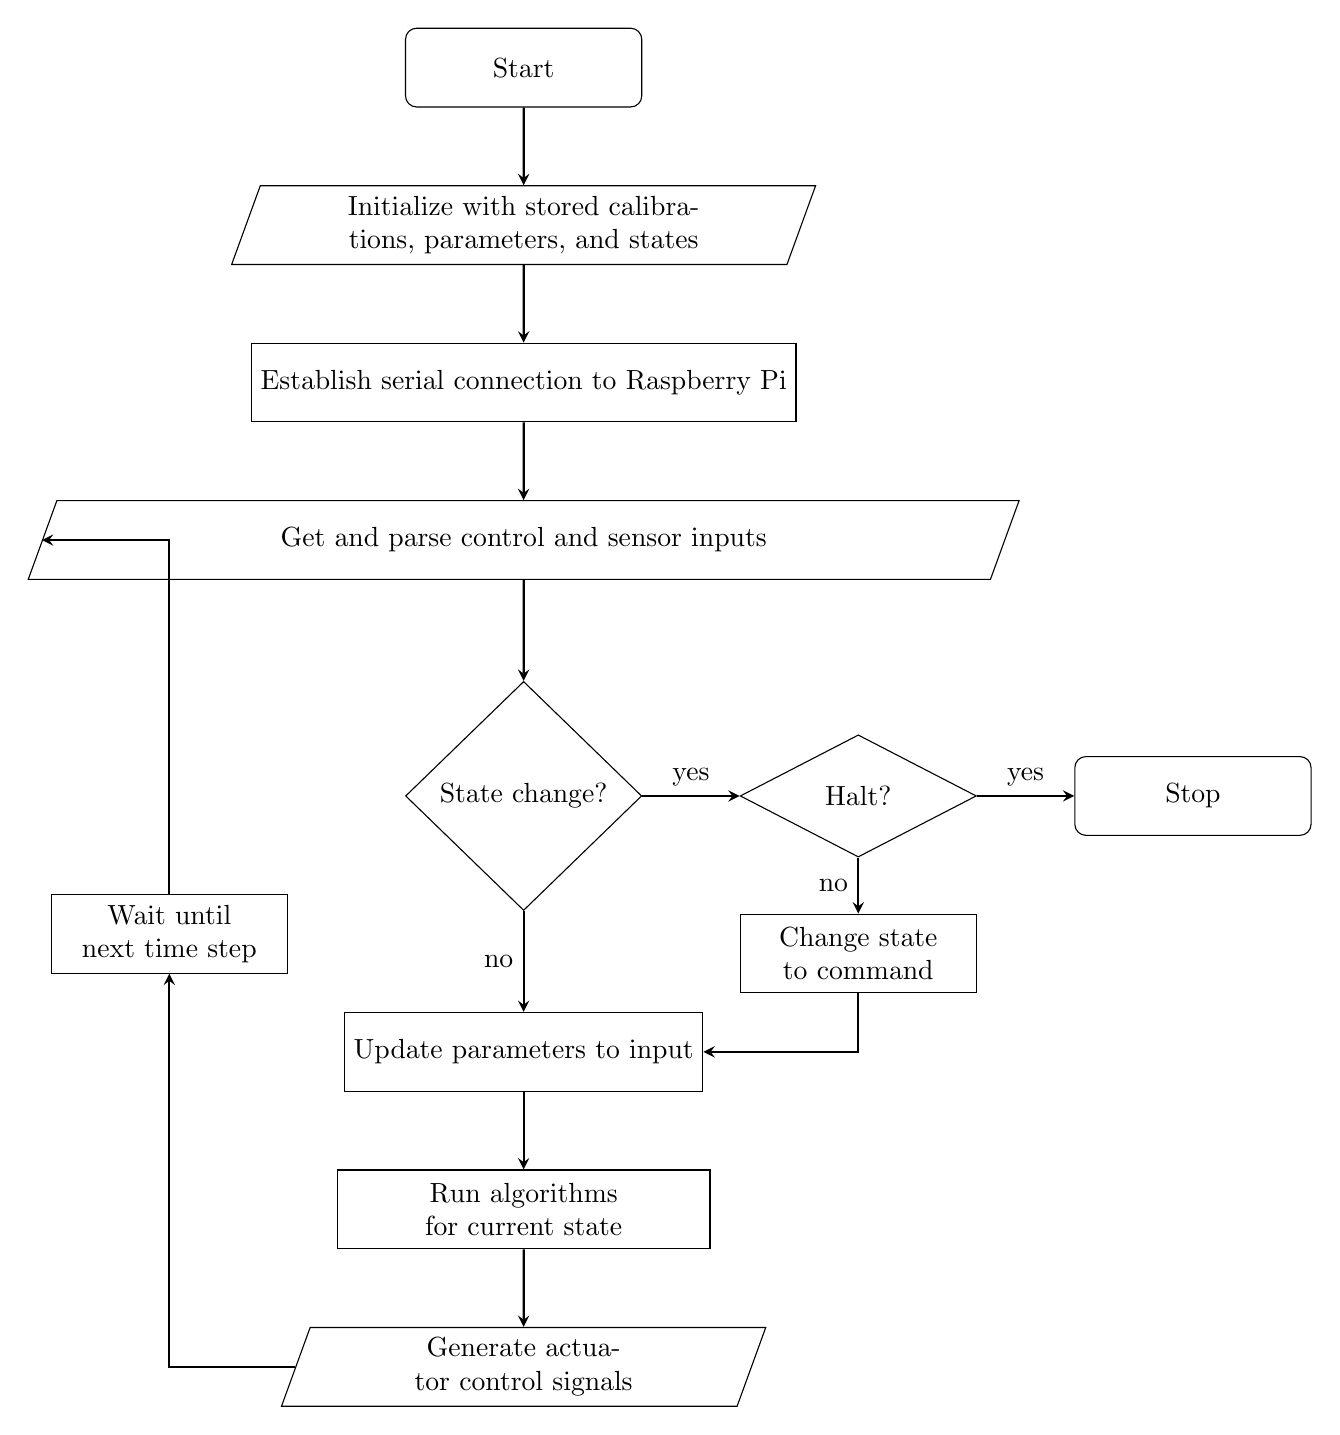
\begin{tikzpicture}[node distance=2cm]

% Nodes / blocks
\node (start) [startstop] {Start};
\node (init) [io, below of=start, text width=6.25cm] {Initialize with stored calibrations, parameters, and states};
\node (estSerial) [process, below of=init] {Establish serial connection to Raspberry Pi};
\node (ctrlInput) [io, below of=estSerial, text width=6.25cm] {Get and parse control and sensor inputs};
\node (ifStateChange) [decision, below of=ctrlInput, yshift=-1.25cm] {State change?};
\node (ifHalt) [decision, right of=ifStateChange, xshift=2.25cm] {Halt?};
\node (stop) [startstop, right of=ifHalt, xshift=2.25cm] {Stop};
\node (stateChange) [process, below of=ifHalt, text width=2.5cm] {Change state to command};
\node (parameterUpdate) [process, below of=ifStateChange, yshift=-1.25cm] {Update parameters to input};
\node (stateProcess) [process, below of=parameterUpdate, text width=4.5cm] {Run algorithms for current state};
\node (controlActuators) [io, below of=stateProcess, text width=5cm] {Generate actuator control signals};
\node (nextTimestep) [process, left of=parameterUpdate, text width=2.5cm, xshift=-2.5cm, yshift=1.5cm] {Wait until next time step};

% Arrows
\draw [arrow] (start) -- (init);
\draw [arrow] (init) -- (estSerial);
\draw [arrow] (estSerial) -- (ctrlInput);
\draw [arrow] (ctrlInput) -- (ifStateChange);
\draw [arrow] (ifStateChange) -- node[anchor=south] {yes} (ifHalt);
\draw [arrow] (ifHalt) -- node[anchor=south] {yes} (stop);
\draw [arrow] (ifHalt) -- node[anchor=east] {no} (stateChange);
\draw [arrow] (ifStateChange) -- node[anchor=east] {no} (parameterUpdate);
\draw [arrow] (stateChange) |- (parameterUpdate);
\draw [arrow] (parameterUpdate) -- (stateProcess);
\draw [arrow] (stateProcess) -- (controlActuators);
\draw [arrow] (controlActuators) -| (nextTimestep);
\draw [arrow] (nextTimestep) |- (ctrlInput);

\end{tikzpicture}



% Results
\newpage
\input{topics/results.tex}


% Future scope
\newpage
\input{topics/futurescope.tex}


% Conclusion
\newpage
\chapter{Conclusion}
Designed and developed a fully functional Quadruped Robot which can map out the environment and perform a range of tasks.


% References
\newpage
\begin{center}
\addcontentsline{toc}{chapter}{References}
\Large \textbf{References}\\
\end{center}


\end{document}